\documentclass[12pt]{article}
\usepackage{graphicx}
\usepackage{amsmath}               % great math stuff
\usepackage{amsfonts}              % for blackboard bold, etc
\usepackage{authblk}

\title{Analyzing the Backlog Bound of Window Flow Controller with Stochastic Network Calculus}

\date{}

\author[a]{Baoliang Li}
\author[b]{Jie Zhao}
\author[a]{Wenhua Dou}

\affil[a]{College of Computer, National University of Defense Technology}
\affil[b]{State Key Laboratory of Mathematical Engineering and Advanced Computing}

\newtheorem{theorem}{Theorem}
\newtheorem{lemma}{Lemma}
\newtheorem{definition}{Definition}
\newtheorem{proof}{Proof}

\hyphenation{DNC}
\hyphenation{SNC}
\hyphenation{WFC}
\hyphenation{DCF}

\begin{document}
\maketitle
\begin{abstract}
Window Flow Controller (WFC) has been widely used in the computer networks and interconnection networks for its simplicity and high efficiency. It is very important to quantify the buffer requirement of the WFC, because the buffer is always a scarce resource and should be allocated on demand. In addition, the stochastic backlog bound can also be viewed as the blocking/loss ratio, which is a key Quality-of-Service (QoS) parameter of the network. To meet this great demand, we study the stochastic backlog bound by leveraging the recently developed Stochastic Network Calculus (SNC) theory. Breaking the dependence between arrived traffic and admitted traffic, and characterizing the stochastic backlog bound with appropriate traffic model and service model are the main task of this paper. The main contribution of our work is the derivation of four stochastic backlog bounds for the lossless WFC, with each bound applying under different condition. The stochastic backlog bounds we obtained in this paper are non-asymptotic, which complements the steady-state results based on queueing theory. Our work not only promotes the theory and application of SNC, but also provides a powerful analytical approach for the performance evaluation and optimization of network with window flow control. Experimental results demonstrate the effectiveness of our proposed backlog bounds.
\end{abstract}

{\bf Keywords:} Window Flow Controller, Stochastic Network Calculus, Backlog Bound

\section{Introduction}
Flow control is an efficient mechanism to avoid network congestion, deadlock and unfair resource allocation \cite{1094691}. Among all these flow control mechanisms, Window Flow Controller (WFC) has been widely used in the computer networks and interconnection networks for its simplicity and high efficiency. The well-known Transmission Control Protocol \cite{RFC5681} and credit-based flow control \cite{372658,DaTo04} are two typical implementations of WFC.\@ In a network with WFC, to realize the lossless transmission, the controller should allocate enough buffer to hold the arrived packets temporarily when the number of unacknowledged packets exceeds the window size.\@ Determining the buffer requirement of lossless WFC is necessary and critical for the following two reasons: (1) The buffer should be allocated on demand, as it is always a scarce resource in any system; (2) The stochastic backlog bound can also be utilized to estimate the blocking/loss ratio for realistic networks, which is a key Quality-of-Service (QoS) parameter. Thus, one question raised: for given WFC parameters, e.g. feedback delay and window size, how to determine the buffer size of the controller under certain arrival and service pattern in order to guarantee certain QoS level? Simulation is commonly used for this purpose, although providing high accuracy, it is very time-consuming and difficult to cover all the configurations. Thus, in this paper, we adopt the analytical approach to evaluate the stochastic backlog bound of WFC.

Our theoretical background is the Stochastic Network Calculus (SNC) \cite{Chan94,jiang2006basic,Ciucu2006Scaling,5984844,Fidl06} theory, which has gained great success in the service guarantee of stochastic service systems. Unfortunately, current SNC theory is mainly focusing on the performance analysis of feed-forward network with infinite buffer capacity, and the analysis of feedback network with SNC has been recognized as a research challenge \cite{JiangLiu-15877}. In this paper, we first establish a relationship between the arrival process and the admitted process in idle period, which allows us to use the arrival process and the service process to characterize the backlog bound of WFC. Then, we derive four backlog bounds based on different probability techniques, each with different accuracy and suitable for different scenarios. Our work can be viewed as the stochastic extension of Deterministic Network Calculus (DNC) based WFC performance analysis \cite{CrOk96,AgRa96,Chan98,ACOR99,QLDD09FC,bose2006analysis,Qian2010Analysis}. The obtained results are more general than those obtained by queueing theory, e.g. \cite{1095377,jung1996analysis}, because the latter method restricts the arrival and service to be Markovian. The main contribution of this paper is the derivation of four stochastic backlog bound for the lossless WFC, with each bound applying under different condition. Our work not only extends the application field of SNC to feedback networks, but also provides a novel analytical approach for the performance evaluation of network with feedback control loop. In addition, we also investigated the impact of various WFC parameters (e.g. window size and feedback delay) on the backlog bound.

The rest of this paper is organized as follows. Section \ref{relate} reviews related work. In section \ref{Notations}, we first introduce the notations and assumptions used in this paper, and then give a brief description of the WFC model. Finally, the theoretical background of SNC and its related theories are presented. Four backlog bounds are derived in section \ref{sncloss} with each applying under different conditions. We present the experiment results to verify our results and illustrate the feasibility of our theorems in section \ref{experiments}. Finally, we summarize this paper in section \ref{concluson}.

\section{Related Work}\label{relate}
Besides the simulation based methods, researchers have proposed various analytical methods to analyze the performance of WFC, e.g. queueing theory \cite{1094531,Chu:1981:ATQ:1310158.1310656,berger1992impact,jung1996analysis,1095377,1092752,113869}, automata \cite{Billington:2007:FTD:1366708.1366712}, petri net \cite{Gaeta2003}, max-plus algebra \cite{BaHo00}, control theory \cite{wang2008internet} and DNC \cite{CrOk96,AgRa96,Chan98,ACOR99,QLDD09FC,bose2006analysis,Qian2010Analysis}, etc. For more information about the modeling and analysis of flow and congestion control, please refer to \cite{srikant2004mathematics}. Among all these theories, DNC and queueing theory are the most commonly adopted theories, both achieve great success in the performance modeling and analysis of WFC. Deterministic network calculus is a theory of deterministic queueing system, it mainly focuses on the worst-case performance bound of WFC, e.g. backlog \cite{QLDD09FC,bose2006analysis}, delay \cite{Qian2010Analysis}. However, the worst-case performance bound is very conservative and usually leads to the over-allocation of network resource, because the occurrence of the worst-case scenarios is usually very rare. Queueing theory is a theory of stochastic service analysis, it mainly focuses on the average performance, e.g. delay, queueing length and utilization, but restricts the arrival and service processes to be Markovian. In addition, just knowing the average or worst-case performance is not enough for the guarantee of QoS. Thus, the stochastic performance modeling and analysis of WFC still remain an open issue.

In this paper, we fill this gap by leveraging the SNC theory, which is a theory for stochastic service guarantee analysis. Stochastic network calculus is a probabilistic extension of DNC, and gives the performance bound in the manner of probability tail distribution. Although introduced in early 1990s \cite{Chan94}, the theory of SNC becomes applicable recently, and several variations have been proposed, e.g. \cite{jiang2006basic,Fidl06,5984844,Ciucu2006Scaling}. Please refer to \cite{JiangLiu-15877} for more details about SNC. For the systems providing stochastic service, SNC can give more reasonable performance bound than DNC, and be feasible to much more general scenarios than queueing theory. Thus, SNC has been widely used in the field of network coding \cite{10.1109/TPDS.2010.192}, cognitive radio \cite{5466711}, 802.11 DCF \cite{xie2010network}\cite{wang2012effectiveness}, wireless fading channel \cite{Fidler2006network,wangperformance}, etc. However, as far as we know, all these existing applications of SNC are limited to feed-forward networks with infinite buffer capacity. Although the retransmission models in \cite{wangperformance,5466711} introduce the feedback from the destination to the source, the influence of feedback is eliminated by applying either the data scaling element \cite{wangperformance} or the impairment process \cite{5466711}. Our work in this paper is the first attempt to applying the SNC theory directly to the performance analysis of feedback networks. The most related work to our research is the queueing theory based analysis and optimization of pacing window flow control \cite{jung1996analysis,1095377}, especially the performance model for sliding window flow control proposed in \cite{jung1996analysis}. In section \ref{experiments} of this paper, we will illustrate that, our theorems not only provide the same backlog bound as in \cite{jung1996analysis} but also complement the results obtained from queueing theory and DNC.

\section{Preliminaries}\label{Notations}
We first outline the notations used in this paper in subsection \ref{notation}, then introduce the flow control model in subsection \ref{model}. Finally, the definition of traffic and service models utilized to derive the backlog bounds are given in subsection \ref{trafficservice}. Two theorems used to obtain the stochastic service models are also proposed in this subsection.

\subsection{Notations}\label{notation}
In this paper, we consider the discrete time network model for simplicity. A process is defined as a non-deceasing casual function on time $t\ (t\geq 0)$. Specifically, denote the accumulative arrival process $\mathcal{A}(t)$ as the amount of traffic (in bits) arrived by time $t$, the accumulative service process $\mathcal{S}(t)$ as the amount of service (in bits) provided by the system by time $t$. Similarly, the accumulative admitted process $\mathcal{I}(t)$ and the accumulative departure process $\mathcal{D}(t)$ denote the amount of traffic entering the system and the amount of traffic departed from the system, respectively. All $\mathcal{A}(t)$, $\mathcal{S}(t)$, $\mathcal{I}(t)$ and $\mathcal{D}(t)$ belong to the set of non-negative non-decreasing functions, denoted by $\mathcal{F}$, and for any function $a(x)\in\mathcal{F}$, let $a(x)=0,\forall x<0$. We also define the following four bivariate functions to simplify our expressions: $\mathcal{A}(s,t)=\mathcal{A}(t)-\mathcal{A}(s)$, $\mathcal{T}(s,t)=\mathcal{T}(t)-\mathcal{A}(s)$, $\mathcal{S}(s,t)=\mathcal{S}(t)-\mathcal{S}(s)$ and $\mathcal{D}(s,t)=\mathcal{D}(t)-\mathcal{D}(s)$. Denote by $\bar{\mathcal{F}}$ the set of non-negative non-increasing functions, and for any function $a(x)\in\bar{\mathcal{F}}$, let $a(x)=1,\forall x<0$. A subset of $\bar{\mathcal{F}}$, denoted by $\bar{\mathcal{G}}$, is defined as, for each function $h(x)\in\bar{\mathcal{G}}$, the $n$th-fold integration ($n\geq 0$), i.e. $(\int_{x}^\infty dy)^nh(y)$, still belongs to $\bar{\mathcal{G}}$. In addition, we leverage the following two notations to shorten our expressions: $[x]_1=\min\{x,1\}$, $[x]^+=\max\{x,0\}$.

The min-plus convolution $\otimes$, de-convolution $\oslash$ and Stieltjes convolution $\ast$ used in this paper are defined as
$$f\otimes g(t)=\min_{0\leq s\leq t}\left\{f(s)+g(t-s)\right\},$$
$$f\oslash g(t)=\sup_{s\geq 0}\left\{f(s+t)-g(s)\right\},$$
$$f\ast g(t)=\int_{-\infty}^{\infty}f(x-y)dg(y).$$

\subsection{Network Model}\label{model}
Flow control is an efficient solution for the networks to prevent the sender from overflowing the buffer of the receiver. In the computer networks, a packet flow generated by a source traverses several intermediate nodes (e.g. switch or router) and terminated at the destination. To prevent buffer overflow, the number of packets \textquoteleft in flight\textquoteright\ should be limited. This is achieved by enforcing the destination return an acknowledgment to the source for each packet that has been correctly received. The source releases a packet whenever the number of unacknowledged packet does not exceed the window size $W$. Besides the TCP \cite{RFC5681} in transmission layer, two typical flow control mechanisms in data link layer, i.e. sliding window and stop-and-wait, can also be viewed as window flow control, corresponding to the $W>1$ and $W=1$ scenarios. Credit-based flow control is another example of WFC, it maintains a counter at the sender to track the buffer available at the receiver. This counter increases when the receiver consumes a cell and decreases when the sender releases a cell.

The closed-loop flow control mechanism discussed above is illustrated in Fig. \ref{control1}, which has been investigated in DNC theory \cite{CrOk96,AgRa96,Chan98,ACOR99,QLDD09FC,bose2006analysis,Qian2010Analysis}. This model is comprised of two sub-systems in tandem, and the second sub-system has finite buffer capacity. The feed-forward service process and feedback service process are denoted as $\mathcal{S}_1(t)$ and $\mathcal{S}_2(t)$, respectively. The feedback process, i.e. number of acknowledgements fed back to the source by time $t$, is denoted as $\mathcal{T}(t)$. If the amount of traffic unacknowledged at time instance $t$ is less than the maximal window size $W$, the traffic arrived at the first sub-system can be departed and injected into the second sub-system immediately, or else, stays in the first sub-system to ensure that the amount of unacknowledged traffic never exceeds $W$. Thus, the accumulative admitted process $\mathcal{I}(t)$ can be described with the following equation
\begin{equation}\label{wfc}
\mathcal{I}(t)=\min\{\mathcal{A}(t),\mathcal{T}(t)+W\}.
\end{equation}
\begin{figure}[ht]
  \centering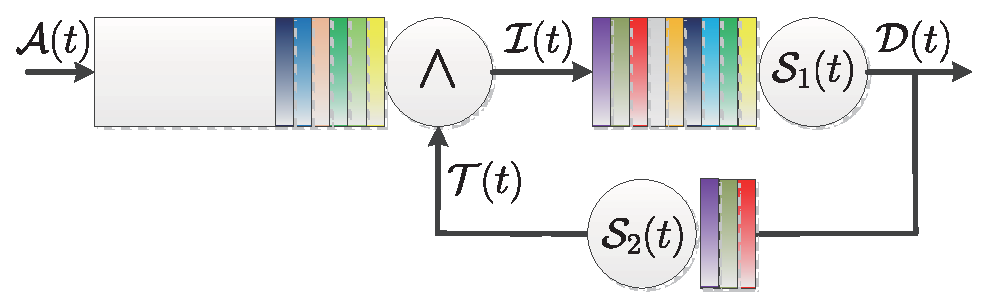
\includegraphics[scale=0.45]{figures/QueueModel1.eps}\\
  \caption{End-to-End Window Flow Control Model}\label{control1}
\end{figure}

We must claim that, although the model presented here is much simpler than the flow control in realistic networks, it is sufficient to demonstrate the key design consideration and the necessary tradeoff that should be made. This model can also be applied to the network with inference traffic, since the services offered to the admitted flow $\mathcal{I}(t)$, i.e. $\mathcal{S}_1(t)$, can be obtained by subtracting the total service capacity provided by the feed-forward network from the services consumed by the inference traffic.

The backlog of controller at time $t$ can be expressed as $$\mathcal{L}(t)=\mathcal{A}(t)-\mathcal{I}(t)$$ and the backlog bound $P\{\mathcal{L}(t)>x\}$ is the probability upper bound that the backlog in the controller at time instance $t$ is greater than $x$. This performance metric is important for the allocation of buffer and the analysis of buffer utilization. This upper bound can also be viewed as the blocking/loss ratio of this system. The backlog bounds we explored in this paper are non-asymptotic, which complements the results obtained with queueing theory based steady-state analysis. Unfortunately, deriving the backlog bound is a non-trival task, this is because there exists dependence between $\mathcal{I}(t)$ and $\mathcal{A}(t)$, as shown in Eq.(\ref{wfc}). In section \ref{sncloss}, we will try to break this dependence and characterize the stochastic backlog bound with appropriate traffic and service model. The traffic and service models we used are presented in the follow subsection.

\subsection{Traffic and Service Models}\label{trafficservice}
In this subsection, we describe the basic concepts of SNC used to derive the backlog bound of window flow controller. Stochastic network calculus is developed for the purpose of stochastic performance analysis. Two fundamental concepts in SNC are stochastic arrival curve and stochastic service curve, both have several variations \cite{JiangLiu-15877,jiang2006basic}.
These two concepts are the stochastic extension of arrival curve and service curve defined in DNC \cite{Boudec2001Network}.

In order to derive the upper bound of backlog of the controller, we have to adopt the $v.b.c.$ stochastic arrival curve \cite{jiang2006basic,JiangLiu-15877} and $v.b.$ stochastic strict service curve \cite{Wu2010Model} to characterize the arrival process and feedback service process, respectively. We only present the definitions of these two models in this subsection due to the space limitation. For more details about these two concepts please refer to \cite{JiangLiu-15877,Wu2010Model,jiang2006basic}.

\begin{definition}[$v.b.c.$ stochastic arrival curve]
A flow $\mathcal{A}(t)$ is said to have a virtual-backlog-centric ($v.b.c.$) stochastic arrival curve $\alpha\in\mathcal{F}$ with bounding function $f\in\bar{\mathcal{F}}$, denoted by $<f,\alpha>$, if for all $t\geq 0$ and all $x\geq 0$, the following inequality holds
$$P\left\{\sup_{0\leq s\leq t}\{\mathcal{A}(s,t)-\alpha(t-s)\}>x\right\}\leq f(x).$$
\end{definition}

\begin{definition}[$v.b.$ stochastic strict service curve]
A system $\mathcal{S}(t)$ is said to have a virtual-backlog ($v.b.$) stochastic strict service curve $\beta\in\mathcal{F}$ with bounding function $g\in\bar{\mathcal{F}}$, denoted by $<g,\beta>$, if for all $x\geq 0$ and $t\geq 0$, the following inequality holds
$$P\left\{\sup_{0\leq s\leq t}\{\beta(t-s)-\mathcal{S}(s,t)\}>x\right\}\leq g(x).$$
\end{definition}

In this paper, we also proposed the concept of $m.b.$ stochastic strict service curve to characterize the feed-forward service process, as shown in the following definition.
\begin{definition}[$m.b.$ stochastic strict service curve]
A system $\mathcal{S}(t)$ is said to have a maximum-backlog ($m.b.$) stochastic strict service curve $\beta\in\mathcal{F}$ with bounding function $g\in\bar{\mathcal{F}}$, denoted by $<g_t,\beta>$, if for all $x\geq 0$ and $t\geq 0$, the following inequality holds
$$P\left\{\sup_{0\leq s\leq t}\sup_{0\leq u\leq s}\{\beta(s-u)-\mathcal{S}(u,s)\}>x\right\}\leq g_t(x).$$
\end{definition}

If we construct a single node queueing system which provides service process $\mathcal{S}$ to the arrival process $\beta(t)$, the maximum backlog of this system can be described as $\sup_{0\leq s\leq t}\sup_{0\leq u\leq s}\{\beta(s-u)-\mathcal{S}(u,s)\}$. That is why we call it as maximum-backlog stochastic strict service curve.

The $v.b.c.$ stochastic arrival curve has been widely used in SNC to derive performance bound, and several methods have been proposed to obtain this curve, e.g. model transform \cite{jiang2006basic,Wu2010Model,JiangLiu-15877}, queueing theory based method \cite{Wu2010Model} and martingale based method \cite{jiang2010note}. However, methods of obtaining the $v.b.$ stochastic strict service curve are not fully discussed in the literature, because it is only proposed to establish a relationship between queueing theory and stochastic service curve \cite{Wu2010Model}. In this paper, we have to leverage the concept of beginning of last backlogged period \cite{Fidl06} to break the dependence between the arrived process and admitted process, and utilize the $v.b.$ and $m.b.$ stochastic service curve to estimate the backlog bound. Before we give the detailed derivation steps, we should first provide some methods which can be used to obtain these two stochastic service curves.

Besides the queueing theory based method proposed in \cite{Wu2010Model} to obtain the $v.b.$ stochastic strict service curve, we find that it has close relationship with stochastic strict service curve \cite{JiangLiu-15877}. So, we propose a model transform based method, i.e. Theorem \ref{mtrans}, to obtain the $v.b.$ stochastic strict service curve from stochastic strict service curve.
\begin{theorem}\label{mtrans}
(1) If a system $\mathcal{S}(t)$ provides a $v.b.$ stochastic strict service curve $\beta(t)\in\mathcal{F}$ with bounding function $g(x)\in\bar{\mathcal{F}}$, the system also provides a stochastic strict service curve with the same service curve and bounding function.

(2) If a system $\mathcal{S}(t)$ provides a stochastic strict service curve $\beta(t)\in\mathcal{F}$ with bounding function $g(x)\in\bar{\mathcal{G}}$ and $\beta_{\theta}(t)=\beta(t)-\theta\cdot t\in\mathcal{F}$ for some $\theta>0$, it also provides a $v.b.$ stochastic strict service curve $\beta_{\theta}(t)$ with bounding function $g_{\theta}(x)=[g(x)+\frac{1}{\theta}\int_x^\infty g(y)dy]_1$ for any $\theta>0$ satisfying $\beta_{\theta}(t)\in\mathcal{F}$.
\end{theorem}

\begin{proof}
(1) Obviously, for any $0\leq s\leq t$, we have
$$\beta(t-s)-\mathcal{S}(s,t)\leq \sup_{0\leq s^\prime\leq t}\left\{\beta(t-s^\prime)-\mathcal{S}(s^\prime,t)\right\}$$
which implies the following inequality
\begin{eqnarray*}
P\left\{\beta(t-s)-\mathcal{S}(s,t)>x\right\} &\leq& P\left\{\sup_{0\leq s^\prime\leq t}\left\{\beta(t-s^\prime)-\mathcal{S}(s^\prime,t)\right\}>x\right\}.
\end{eqnarray*}
The left side of this inequality corresponds to the stochastic strict service curve. Thus, the bounding function of $v.b.$ stochastic strict service curve is indeed a bounding function for the stochastic strict service curve with the same stochastic strict service curve.

(2) If a system $\mathcal{S}(t)$ provides a stochastic strict service curve $\beta(t)$ with bounding function $g\in\bar{\mathcal{G}}$, and $\beta(t)-\theta \cdot t\in\mathcal{F}$, where $\theta>0$ is a free parameter, then, for any $\theta$ satisfying $\beta_{\theta}(t)\in\mathcal{F}$, we can construct a $v.b.$ stochastic strict service curve $\beta_{\theta}(t)=\beta(t)-\theta \cdot t$. The bounding function of $\beta_\theta(t)$ can be obtained following the same procedure of Theorem 3.13 in \cite{JiangLiu-15877}, which is
\begin{eqnarray*}
P\left\{\sup_{0\leq s\leq t}\{\beta_{\theta}(t-s)-\mathcal{S}(s,t)\}>x\right\} &= &P\left\{\sup_{0\leq s\leq t}[\beta_{\theta}(t-s)-\mathcal{S}(s,t)]^+>x\right\}\\
&\leq &\sum_{s=0}^t P\left\{[\beta_{\theta}(t-s)-\mathcal{S}(s,t)]^+>x\right\}\\
&\leq &\sum_{s=0}^t g(x+\theta\cdot(t-s))\\
&\leq & \sum_{\tau=0}^\infty g(x+\theta\tau)\\
&\leq & g(x)+\frac{1}{\theta}\int_{x}^\infty g(y)dy
\end{eqnarray*}
which completes the proof.
\end{proof}

We can also derive the model transform theorem between $v.b.$ stochastic strict service curve and $m.b.$ stochastic strict service curve, as shown in the following theorem, which provides a way to obtain the $m.b.$ stochastic strict service curve. We omit the detailed proof of this theorem, since it can be easily proved following the same proof procedure as Theorem \ref{mtrans}.
\begin{theorem}\label{mtrans2}
(1) If a system $\mathcal{S}(t)$ provides a $m.b.$ stochastic strict service curve $\beta(t)\in\mathcal{F}$ with bounding function $g(x)\in\bar{\mathcal{F}}$, the system also provides a $v.b.$ stochastic strict service curve with the same service curve and bounding function.

(2) If a system $\mathcal{S}(t)$ provides a $v.b.$ stochastic strict service curve $\beta(t)\in\mathcal{F}$ with bounding function $g(x)\in\bar{\mathcal{G}}$ and $\beta_{\theta}(t)=\beta(t)-\theta\cdot t\in\mathcal{F}$ for some $\theta>0$, it also provides a $m.b.$ stochastic strict service curve $\beta_{\theta}(t)$ with bounding function $g_{\theta}(x)=[g(x)+\frac{1}{\theta}\int_x^\infty g(y)dy]_1$ for any $\theta>0$ satisfying $\beta_{\theta}(t)\in\mathcal{F}$.
\end{theorem}

Stochastic network calculus utilizes stochastic arrival curve and stochastic service curve to describe the arrival and service process, and derive the performance bound based on some basic probability techniques. It usually does not make any assumption on the arrival and service processes, making it feasible to wide range of applications. However, for some specific conditions, much tighter bound can be obtained if some advance probability techniques, e.g. effective bandwidth, effective capacity and martingale theory, are integrated into the analysis framework, e.g. \cite{Li2007Network,5984844,jiang2009network,Ciucu2007Network}. Hence, we present the concepts of effective bandwidth \cite{Kelly1996Note} and effective capacity \cite{Wu2003Effective} used to derive the backlog bound when the arrival and service processes are stationary.
\begin{definition}[Effective Bandwidth and Effective Capacity]
The effective bandwidth with respect to a flow is defined as
$$\rho(\theta_a,t_a)=\frac{1}{\theta_a t_a}log E[e^{\theta_a \mathcal{A}(t_a)}]$$
where the parameters $\theta_a>0$ and $t_a<\infty$ are called the space parameter and time parameter, respectively. Similarly, the effective capacity of service process $\mathcal{S}(t_s)$ is defined as
$$\mu^\prime(\theta_s,t_s)=\frac{1}{-\theta_s t_s}log E[e^{-\theta_s \mathcal{S}(t_s)}]$$
where the parameters $\theta_s>0$ and $t_s>0$ are called space parameter and time parameter, respectively.
\end{definition}

Based on the above definitions, we have $E[e^{\theta_a \mathcal{A}(t_a)}]=e^{\theta_a t_a\rho(\theta_a,t_a)}$ and
$E[e^{-\theta_s \mathcal{S}(t_s)}]=e^{-\theta_b t_s\mu^\prime(\theta_s,t_s)}$ which will be used in section \ref{sncloss} to derive the backlog bound of WFC.

\section{Backlog Bound of Window Flow Controller}\label{sncloss}
In this section, we will take up the challenge to derive stochastic backlog bound for the lossless WFC. The backlog bound of the WFC is closely related with arrival process $\mathcal{A}(t)$, the window size $W$, feed-forward service process $\mathcal{S}_1(t)$ and feedback service process $\mathcal{S}_2(t)$, which makes the modeling and analysis very difficult and complex.

We first list the necessary Lemmas in subsection \ref{neclemma}. Based on these Lemmas, we derive four backlog bounds for the WFC in subsection \ref{backlog}.
\subsection{Necessary Lemmas}\label{neclemma}
The following two Lemmas will be used in our derivation to evaluate the tail distribution of random variables. These two Lemmas have been verified in \cite{jiang2006basic}.
\begin{lemma}\label{lamma1}
For any random variable $X$ and any real number $x\geq 0$, we have $$P\{[X]^+>x\}=P\{X>x\}.$$
\end{lemma}

\begin{lemma}\label{lamma3}
For any two random variables $X$ and $Y$, and any real number $x\geq 0$, there holds
$$P\{X+Y>x\}\leq f\otimes g(x)$$
if $P\{X>x\}\leq f(x)$, $P\{Y>x\}\leq g(x)$ and $f(x),g(x)\in\bar{\mathcal{F}}$.

Furthermore, if $X$ and $Y$ are independent, there holds
$$P\left\{X+Y>x\right\}\leq 1-\bar{f}\ast\bar{g}(x)$$
where $\bar{f}(x)=1-[f(x)]_1$ and $\bar{g}(x)=1-[g(x)]_1$.
\end{lemma}

When analyze the queueing system with network calculus theory, we can replace the service elements in the tandem with a equivalent service element providing the same amount of services as the tandem service elements. This allowed us to simplify the flow control model shown in Fig. \ref{control1}, as illustrated in Fig. \ref{control2}. The following Lemma establishes the relationship between the admitted process and the arrival process of simplified flow control model shown in Fig. \ref{control2} in idle period, which serves as the basis for our further derivation.
\begin{figure}[ht]
  \centering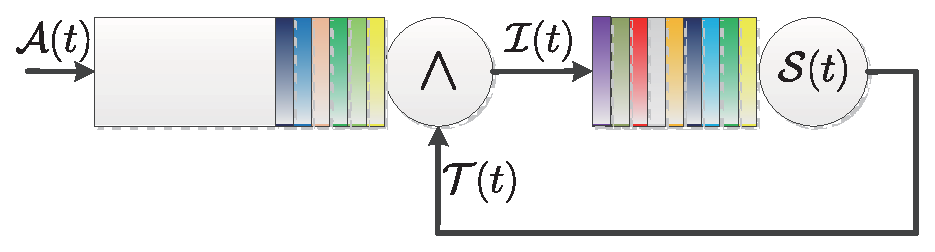
\includegraphics[scale=0.45]{figures/QueueModel2.eps}\\
  \caption{End-to-End Flow Control}\label{control2}
\end{figure}

\begin{lemma}[Flow Control Principle]\label{lama1}
If $t_0$ is in one of the idle period of lossless WFC shown in Fig. \ref{control2}, $\mathcal{A}(t)$ and $\mathcal{I}(t)$ are the arrival process and admitted process, respectively. Then, we have
\begin{equation}
\mathcal{I}(t_0)=\mathcal{A}(t_0).
\end{equation}
\end{lemma}
\begin{proof}
Obviously, for $\forall t\geq 0$, $\mathcal{I}(t)\leq \mathcal{A}(t)$ by casuality. At time instance $t_0$, if $\mathcal{I}(t_0)<\mathcal{A}(t_0)$, buffered data in controller will be admitted and makes the WFC keep on working, which is contrary to the fact that $t_0$ is in the idle period. Thus, $\mathcal{I}(t_0)=\mathcal{A}(t_0)$.
\end{proof}

We can also get the following Lemma. This Lemma makes no assumptions on the arrival process and service process, and serves as the basis to derive all the four backlog bounds in subsection \ref{backlog}.
\begin{lemma}\label{lama2}
Let $\mathcal{A}(t)$ and $\mathcal{T}(t)$ be the arrival process and feedback process, $W$ be the window size. Then, the backlog bound
$$P\{\mathcal{L}(t)> x\}=P\{\mathcal{A}(t)-\mathcal{T}(t)-W> x\}.$$
\end{lemma}
\begin{proof}
As shown in Fig. \ref{control2}, for any sample path $\mathcal{A}(t)$ and $\mathcal{T}(t)$, the backlog $\mathcal{L}(t)$ in WFC can be expressed as
\begin{eqnarray}
  \mathcal{L}(t)&=&\mathcal{A}(t)-\mathcal{I}(t)\nonumber\\
      &=&\mathcal{A}(t)-\min\{\mathcal{A}(t),\mathcal{T}(t)+W\}\nonumber\\
      &=&[\mathcal{A}(t)-\mathcal{T}(t)-W]^+.\nonumber
\end{eqnarray}

According to Lemma \ref{lamma1}, we have
\begin{eqnarray*}
  P\{\mathcal{L}(t)>x\}&=&P\{[\mathcal{A}(t)-\mathcal{T}(t)-W]^+>x\}\\
  &=&P\{\mathcal{A}(t)-\mathcal{T}(t)-W>x\}
\end{eqnarray*}
which ends the proof.
\end{proof}

\subsection{Backlog Bound}\label{backlog}
In this subsection, we will try to break the dependence between arrived traffic $\mathcal{A}(t)$ and admitted traffic $\mathcal{I}(t)$, and provide four backlog bounds for the WFC, each with different applying conditions.
\begin{theorem}\label{theorem1}
For a WFC with window size $W$, suppose the arrival process $\mathcal{A}(t)$ has a $v.b.c.$ stochastic arrival curve $<f,\alpha>$, the feed-forward service process $\mathcal{S}_1(t)$ has a $m.b.$ stochastic strict service curve $<g_1,\beta_1>$ and the feedback service process $\mathcal{S}_2(t)$ provides a $v.b.$ stochastic strict service curve $<g_2,\beta_2>$. When $\lim_{t\to\infty}\{\alpha(t)-\beta_1\otimes\beta_2(t)\}/t\leq 0$, the backlog $\mathcal{L}(t)$ in the WFC is bounded by
\begin{equation}\label{eqn1}
P\left\{\mathcal{L}(t)>x\right\}\leq [f\otimes g_1\otimes g_2([y^\prime]^+)]_1
\end{equation}
where $y^\prime=x+W-\sup_{0\leq v\leq t}\{\alpha\oslash(\beta_1\otimes\beta_2)(v)\}$.

If $\mathcal{A}(t)$, $\mathcal{S}_1(t)$ and $\mathcal{S}_2(t)$ are independent, we can get a much tighter backlog bound with Stieljes convolution
\begin{equation}\label{eqn2}
P\{\mathcal{L}(t)>x\}\leq 1-\bar{f}\ast\bar{g}_1\ast\bar{g}_2([y^\prime]^+).
\end{equation}
\end{theorem}

\begin{proof}
enlightened by Lemma \ref{lama2}, to evaluate $P\{\mathcal{L}(t)>x\}$, we can estimate $P\{\mathcal{A}(t)-\mathcal{T}(t)-W>x\}$ first.

For the simplified model shown in Fig. \ref{control2}, denote by $t_{0}$ the beginning of last backlogged period before $t$ \cite{Fidl06}, i.e. $t_0=\sup\{s\in[0,t]:\mathcal{I}(s)=\mathcal{T}(s)\}$, then $0\leq t_{0}\leq t$. By applying Lemma \ref{lama1}, we have
\begin{eqnarray*}
  \mathcal{T}(t)&=&\mathcal{I}(t_{0})+\mathcal{S}(t_{0},t)\\
  &=& \mathcal{A}(t_{0})+\mathcal{S}(t_{0},t).
\end{eqnarray*}

Hence,
\begin{eqnarray}
\mathcal{L}(t)&=&\mathcal{A}(t)-\mathcal{T}(t)-W\nonumber\\
&=&\mathcal{A}(t_0,t)-\mathcal{S}(t_0,t)-W\label{used4theorem5}\\
&=&\mathcal{A}(t_0,t)-\mathcal{T}(t_0,t)-W\nonumber.
\end{eqnarray}

Denote by $t_1$ the beginning of last backlogged period of sub-system $\mathcal{S}_2(t)$ before $t$, then
$$\mathcal{T}(t)=\mathcal{D}(t_1)+\mathcal{S}_2(t_1,t).$$

Since $\mathcal{T}(t_0)=\mathcal{D}(t_0)$, we have
\begin{eqnarray}
\mathcal{A}(t_0,t)-\mathcal{T}(t_0,t) &=& \mathcal{A}(t_0,t)-\mathcal{T}(t)+\mathcal{T}(t_0)\nonumber\\
&=& \mathcal{A}(t_0,t)-\mathcal{S}_2(t_1,t)-\mathcal{D}(t_0,t_1).\label{start}
\end{eqnarray}

Let $t_2$ be the beginning of last backlogged period of $\mathcal{S}_1(t)$ before $t_1$, then $t_0\leq t_2< t_1$ and
\begin{eqnarray}
\mathcal{A}(t_0,t)-\mathcal{S}_2(t_1,t)-\mathcal{D}(t_0,t_1) &=& \mathcal{A}(t_0,t)-\mathcal{S}_2(t_1,t)-\mathcal{D}_1(t_0,t_2)-\mathcal{S}_1(t_2,t_1)\nonumber\\
&\leq& \mathcal{A}(t_0,t)-\mathcal{S}_2(t_1,t)-\mathcal{S}_1(t_2,t_1)\label{used4effec}\\
&=& [\mathcal{A}(t_0,t)-\alpha(t-t_0)]\nonumber\\
&& +[\beta_1(t_1-t_2)-\mathcal{S}_1(t_2,t_1)]\nonumber\\
&& +[\beta_2(t-t_1)-\mathcal{S}_2(t_1,t)]\nonumber\\
&& +[\alpha(t-t_0)-\beta_1(t_1-t_2)-\beta_2(t-t_1)].\label{initial}
\end{eqnarray}

For the expression in the last square brackets, let $s=t_{1}-t_{2}$ and $u=t_{2}-t_{0}$, then $0\leq s\leq t$ and $0\leq u\leq t$. We also have
\begin{eqnarray}
  \alpha(t-t_{0})-\beta_1(t_{1}-t_{2})-\beta_2(t-t_1)&\leq &\alpha(t-t_{0})-\inf_{0\leq s\leq t}\{\beta_1(s)+\beta_2(t-t_2-s)\}\nonumber\\
  &=&\alpha(t-t_{0})-\beta_1\otimes\beta_2(t-t_{2})\nonumber\\
  &=&\alpha(t-t_{0})-\beta_1\otimes\beta_2(t-t_{0}-u)\nonumber\\
  &\leq & \sup_{0\leq u\leq t-t_0}\{\alpha(t-t_0)-\beta_1\otimes\beta_2(t-t_0-u)\}\nonumber\\
  &\leq& \alpha\oslash(\beta_1\otimes\beta_2)(u)\nonumber\\
  &\leq & \sup_{0\leq v\leq t}\{\alpha\oslash(\beta_1\otimes\beta_2)(v)\}.\label{curve}
\end{eqnarray}

Denote by $\mathcal{Y}_1(t)=\sup_{0\leq s\leq t}\sup_{0\leq u\leq s}\{\beta_1(s-u)-\mathcal{S}_1(u,s)\}$, $\mathcal{Y}_2(t)=\sup_{0\leq s\leq t}\{\beta_2(t-s)-\mathcal{S}_2(s,t)\}$ and $\mathcal{X}(t)=\sup_{0\leq s\leq t}\{\mathcal{A}(s,t)-\alpha(t-s)\}$, we have
\begin{equation}\label{vbc}
\mathcal{A}(t_{0},t)-\alpha(t-t_{0})\leq \mathcal{X}(t),
\end{equation}
\begin{equation}\label{mb}
\beta_1(t_1-t_{2})-\mathcal{S}_1(t_{2},t_1)\leq \mathcal{Y}_1(t)
\end{equation}
and
\begin{equation}\label{vb}
\beta_2(t-t_{1})-\mathcal{S}_2(t_{1},t)\leq \mathcal{Y}_2(t).
\end{equation}

Combining Eq.(\ref{start})-Eq.(\ref{vb}), we get
\begin{eqnarray*}
\mathcal{A}(t_0,t)-\mathcal{T}(t_0,t) &\leq& \mathcal{X}(t)+\mathcal{Y}_1(t)+\mathcal{Y}_2(t)+\sup_{0\leq v\leq t}\{\alpha\oslash(\beta_1\otimes\beta_2)(v)\}.
\end{eqnarray*}

This inequality is sufficient to obtain the upper bound of $P\{\mathcal{A}(t_0,t)-\mathcal{T}(t_0,t)-W>x\}$, because event $\{\mathcal{A}(t_0,t)-\mathcal{T}(t_0,t)-W>x\}$ implies $\{\mathcal{X}(t)+\mathcal{Y}_1(t)+\mathcal{Y}_2(t)+\sup_{0\leq v\leq t}\{\alpha\oslash(\beta_1\otimes\beta_2)(v)\}-W\}$. Thus, we have
$$P\{\mathcal{A}(t_0,t)-\mathcal{T}(t_0,t)-W>x\}\leq P\{\mathcal{X}(t)+\mathcal{Y}_1(t)+\mathcal{Y}_2(t)>y^\prime\}$$
where $y^\prime=x+W-\sup_{0\leq v\leq t}\{\alpha\oslash(\beta_1\otimes\beta_2)(v)\}$. To keep the system stable, the following condition should be satisfied:
$$\lim_{t\to \infty}\frac{1}{t}\{\alpha(t)-\beta_1\otimes\beta_2(t)\}\leq 0.$$

We also notice that, we can provide a bound for $P\{\mathcal{X}(t)+\mathcal{Y}_1(t)+\mathcal{Y}_2(t)>y^\prime\}$ by leveraging Lemma \ref{lamma3}. Because $P\{\mathcal{X}(t)>y^\prime\}$, $P\{\mathcal{Y}_1(t)>y^\prime\}$ and $P\{\mathcal{Y}_2(t)>y^\prime\}$ are closely related to the $v.b.c.$ stochastic arrival curve, $m.b.$ stochastic strict service curve and $v.b.$ stochastic strict service curve. But, we have to consider the following two cases according to the sign of $y^\prime$.

(1) $y^\prime\geq 0$. Based on the definition of $v.b.c.$ stochastic arrival curve, $m.b.$ stochastic strict service curve and $v.b.$ stochastic strict service curve, we get
$$P\{\mathcal{X}(t)>y^\prime\}\leq f(y^\prime),$$
$$P\{\mathcal{Y}_1(t)>y^\prime\}\leq g_1(y^\prime)$$
and
$$P\{\mathcal{Y}_2(t)>y^\prime\}\leq g_2(y^\prime).$$

By applying Lemma \ref{lamma3}, we have
\begin{equation}\label{equation1}
P\{\mathcal{X}(t)+\mathcal{Y}_1(t)+\mathcal{Y}_2(t)>y^\prime\}\leq f\otimes g_1\otimes g_2(y^\prime).
\end{equation}

(2) $y^\prime<0$. Because $\mathcal{X}(t)\geq 0$, $\mathcal{Y}_1(t)\geq 0$ and $\mathcal{Y}_2(t)\geq 0$, we have
$$P\{\mathcal{X}(t)>y^\prime\}=P\{\mathcal{X}(t)\geq 0\}\leq f(0).$$
$$P\{\mathcal{Y}_1(t)>y^\prime\}=P\{\mathcal{Y}_1(t)\geq 0\}\leq g_1(0)$$
and
$$P\{\mathcal{Y}_2(t)>y^\prime\}=P\{\mathcal{Y}_2(t)\geq 0\}\leq g_2(0).$$

Thus,
\begin{equation}\label{equation2}
P\{\mathcal{X}(t)+\mathcal{Y}_1(t)+\mathcal{Y}_2(t)>y^\prime\}\leq f\otimes g_1\otimes g_2(0).
\end{equation}

Combining these two cases, we have
\begin{eqnarray*}
  P\{\mathcal{L}(t)>x\}&=&P\{\mathcal{A}(t)-\mathcal{T}(t)-W>x\}\\
  &\leq&P\{\mathcal{X}(t)+\mathcal{Y}_1(t)+\mathcal{Y}_2(t)>y^\prime\}\\
  &\leq& f\otimes g_1\otimes g_2([y^\prime]^+).
\end{eqnarray*}

If $\mathcal{A}(t)$, $\mathcal{S}_1(t)$ and $\mathcal{S}_2(t)$ are independent, we can adopt the Stieltjes convolution to get a much tighter probability bound
$$P\{\mathcal{L}(t)>x\}\leq 1-\bar{f}\ast\bar{g_1}\ast\bar{g_2}([y^\prime]^+)$$
which ends the proof.
\end{proof}

The above theorem was derived based on some basic probability techniques without making any assumption on the arrival process and service process. Although generality, the backlog bound can be further improved if we take the characterization of arrival and service into consideration. As shown in the following two theorems.
\begin{theorem}\label{theorem2}
For a WFC with window size $W$, if the arrival process $\mathcal{A}(t)$, feed-forward service process $\mathcal{S}_1(t)$ and feedback service process $\mathcal{S}_2(t)$ are both stationary processes, the backlog bound
$$P\{\mathcal{L}(t)>x\}\leq {t+2\choose 3}\cdot \inf_{\theta\in\Theta}\{\sup_{0\leq w\leq t}e^{\theta((t\rho)\oslash((t\mu_1^\prime)\otimes(t\mu_2^\prime))(\theta,w)-W-x)}\}$$
where $\rho(\theta,t)$ is the effective bandwidth of arrival process, $\mu_1^\prime(\theta,t)$ and $\mu_2^\prime(\theta,t)$ are effective capacity of $\mathcal{S}_1(t)$ and $\mathcal{S}_2(t)$, $\Theta$ is the set of $\theta$ satisfying $\rho(\theta,t)\leq \mu_1^\prime\otimes\mu_2^\prime(\theta,t)$.
\end{theorem}

\begin{proof}
Denote by $t_0$ the beginning of last backlogged period of the simplified flow control model before $t$, $t_1$ the beginning of last backlogged period of sub-system $\mathcal{S}_2(t)$ before $t$ and $t_2$ the beginning of last backlogged period of $\mathcal{S}_1(t)$ before $t_1$. As have been proved in Theorem \ref{theorem1} (see Eq. (\ref{used4effec})),
$$\mathcal{A}(t_0,t)-\mathcal{T}_2(t_0,t) \leq \mathcal{A}(t_0,t)-\mathcal{S}_2(t_1,t)-\mathcal{S}_1(t_2,t_1).$$

Thus,
\begin{eqnarray*}
\lefteqn{P\{\mathcal{L}(t)>x\}}\\
&=&P\{\mathcal{A}(t_0,t)-\mathcal{T}(t_0,t)-W>x\}\\
&\leq&P\{\mathcal{A}(t_0,t)-\mathcal{S}_2(t_1,t)-\mathcal{S}_1(t_2,t_1)-W>x\}\\
&=&P\{e^{\theta(\mathcal{A}(t_0,t)-\mathcal{S}_2(t_1,t)-\mathcal{S}_1(t_2,t_1))}>e^{\theta(W+x)}\}\\
&\leq& e^{-\theta (W+x)}\cdot E[e^{\theta(\mathcal{A}(t_0,t)-\mathcal{S}_2(t_1,t)-\mathcal{S}_1(t_2,t_1))}]\\
&\leq& e^{-\theta (W+x)}\cdot E[\sup_{0\leq u_0\leq u_2\leq u_1\leq t}e^{\theta(\mathcal{A}(u_0,t)-\mathcal{S}_2(u_1,t)-\mathcal{S}_1(u_2,u_1))}]\\
&\leq& e^{-\theta (W+x)}\cdot \sum_{u_1=0}^t\sum_{u_1=u_0} ^t\sum_{u_2=u_0}^{u_1}E[e^{\theta(\mathcal{A}(u_0,t)-\mathcal{S}_2(u_1,t)-\mathcal{S}_1(u_2,u_1))}]\\
&=& e^{-\theta (W+x)}\cdot {t+2\choose 3}\cdot e^{\theta((t-u_0)\rho(\theta,t-u_0)-(u_1-u_2)\mu_1^\prime(\theta,u_1-u_2)-(t-u_1)\mu_2^\prime(\theta,t-u_1))}.
\end{eqnarray*}

Let $s=u_1-u_2$ and $v=u_2-u_0$, then
\begin{eqnarray*}
\lefteqn{e^{\theta((t-u_0)\rho(\theta,t-u_0)-(u_1-u_2)\mu_1^\prime(\theta,u_1-u_2)-(t-u_1)\mu_2^\prime(\theta,t-u_1))}}\\
&\leq & e^{\theta((t-u_0)\rho(\theta,t-u_0)-\inf_{0\leq s\leq t}\{s\mu_1^\prime(\theta,s)-(t-u_2-s)\mu_2^\prime(\theta,t-u_2-s)\})}\\
&=& e^{\theta((t-u_0)\rho(\theta,t-u_0)-(t\mu_1^\prime)\otimes(t\mu_2^\prime)(\theta,t-u_2))}\\
&\leq & e^{\theta(\sup_{v\geq 0}\{(t-u_0)\rho(\theta,t-u_0)-(t\mu_1^\prime)\otimes(t\mu_2^\prime)(\theta,t-u_2)\})}\\
&=& e^{\theta((t\rho)\oslash((t\mu_1^\prime)\otimes(t\mu_2^\prime))(\theta,u_2-u_0))}\\
&\leq& \sup_{0\leq w\leq t}e^{\theta((t\rho)\oslash((t\mu_1^\prime)\otimes(t\mu_2^\prime))(\theta,w))}.
\end{eqnarray*}

Hence
\begin{equation}\label{target}
P\{\mathcal{L}(t)>x\}\leq {t+2\choose 3}\cdot \sup_{0\leq w\leq t}e^{\theta((t\rho)\oslash((t\mu_1^\prime)\otimes(t\mu_2^\prime))(\theta,w)-W-x)}.
\end{equation}

Because the model we considered in this paper is lossless, to avoid infinite backlog, the following stability condition should be hold for $\forall t>0$,
$$\rho(\theta,t)\leq \mu_1^\prime\otimes\mu_2^\prime(\theta,t).$$

Denote by $\Theta$ the set of $\theta$ satisfying $\rho(\theta,t)\leq \mu_1^\prime\otimes\mu_2^\prime(\theta,t)$, then we can optimize the backlog bound by selecting appropriate $\theta\in\Theta$ to make the right-hand side of Eq. (\ref{target}) minimized, which ends the proof.
\end{proof}

\begin{theorem}\label{theorem3}
For the simplified WFC with window size $W$ shown in Fig. \ref{control2}, if the arrival process $\mathcal{A}(t)$ and service process $\mathcal{S}(t)$ are both independent and stationary increment processes, an exact distribution of backlog bound can be obtained by leverage the Doob's martingale inequality
\begin{equation}\label{eqn3}
P\left\{\mathcal{L}(t)>x\right\}\leq \inf_{\theta\in\Theta}\{e^{-\theta(W+x)}\cdot E[e^{\theta(\mathcal{A}(1)-\mathcal{S}(1))}]\}.
\end{equation}
where $\Theta$ is the set of $\theta$ satisfying $E[e^{\theta(\mathcal{A}(1)-\mathcal{S}(1))}]\leq 1$.
\end{theorem}
\begin{proof}
As has been proved in \cite{jiang2009network,Ciucu2007Network}, when arrival process $\mathcal{A}(t)$ and service process $\mathcal{S}(t)$ are independent and stationary increments process, and satisfy $E[e^{\theta(\mathcal{A}(1)-\mathcal{S}(1))}]\leq 1$, stochastic process $\{e^{\theta[\mathcal{A}(t-v,t)-\mathcal{S}(t-v,t)]},1\leq v\leq t\}$ is a supermartingale.

For the simplified network model shown in Fig. \ref{control2}, denote by $t_{0}$ the beginning of last backlogged period before $t$, we have proved in Theorem \ref{theorem1} that
$$\mathcal{L}(t)=\mathcal{A}(t_0,t)-\mathcal{S}(t_0,t)-W.$$

Hence
\begin{eqnarray*}
P\left\{\mathcal{L}(t)>x\right\}  &=&P\left\{\mathcal{A}(t_{0},t)-\mathcal{S}(t_{0},t)-W>x\right\}\\
  &\leq& P\left\{\sup_{0\leq s\leq t}\{\mathcal{A}(s,t)-\mathcal{S}(s,t)\}>W+x\right\}\\
  &=& P\left\{\sup_{0\leq s< t}e^{\theta\{\mathcal{A}(s,t)-\mathcal{S}(s,t)\}}>e^{\theta(W+x)}\right\}\\
  &=& P\left\{\sup_{1\leq v\leq t}e^{\theta\{\mathcal{A}(t-v,t)-\mathcal{S}(t-v,t)\}}>e^{\theta(W+x)}\right\}\\
  &\leq& e^{-\theta(W+x)}\cdot E[e^{\theta\{\mathcal{A}(t-1,t)-\mathcal{S}(t-1,t)\}}]\\
  &=& e^{-\theta(W+x)}\cdot E[e^{\theta(\mathcal{A}(1)-\mathcal{S}(1))}].
\end{eqnarray*}

We can optimize this bound by free parameter $\theta$ under the constraint $E[e^{\theta(\mathcal{A}(1)-\mathcal{S}(1))}]\leq 1$.
\end{proof}

It is highlighted that the backlog bound obtained with Theorem \ref{theorem3}, i.e. the right-hand side of Eq. (\ref{eqn3}), is
independent on time $t$, which indicates that it is also a steady-state bound.

\section{Numerical Results}\label{experiments}
In this section, we compare the numerical results of backlog bounds calculated with our theorems with experimental and existing theoretical results. Our goals in this section are two-fold: (1) We try to demonstrate the feasibility of our theorems and the tightness of our results; (2) We intend to illustrate the impact of different offered load and window control parameters, e.g. window size and feedback delay, on the backlog bound of WFC. To achieve these goals, we take the credit-based flow controller as an example which is widely used in interconnection networks \cite{DaTo04}. In credit-based flow controller, a dedicated physical link is used to transmit the feedback credit. This dedicated physical link can be modelled as a Latency-Rate (LR) server \cite{StVa98} with service rate $C_2$ and latency $\tau$. Three arrival and service processes combinations are considered in this section: (1) Scenario I: Poisson input and constant rate service; (2) Scenario II: Poisson input with exponentially distributed service time; (3) Scenario III: Bernoulli input and exponentially distributed service time. The reason of choosing these three models is that there are already extensive research results for these models, which can be directly used to derive our backlog bounds.

\subsection{Scenario I}
Under Scenario I, suppose all the packets in the traffic flow have the same length $L$, and the packet arrivals subject to Poisson process with parameter $\lambda$. Then, the traffic has a $v.b.c.$ stochastic arrival curve $<e^{-\theta_1^\prime\theta_1}e^{-\theta_1 x},\frac{\lambda}{\theta_1}(e^{\theta_1 L}-1)\cdot t+\theta_1^\prime\cdot t>$ \cite{jiang2010note}, where $\theta_1^\prime\geq 0$ and $\theta_1>0$ are free parameters. The feed-forward service element is a constant rate server with service rate $C_1$. Then, it can be verified that the constant rate server provides a $m.b.$ stochastic strict service curve $<0,C_1\cdot [t-0]^+>$ and the fixed latency element provides a $v.b.$ stochastic strict service curve $<0,C_2[t-\tau]^+>$.

Let free parameter $\theta_1^\prime=0$, we can get the backlog bound of WFC with Eq.(\ref{eqn2}), which is
\begin{eqnarray}\label{bounding}
P\{\mathcal{L}(t)>x\}&\leq& f\otimes g_1\otimes g_2([x+W-\alpha\oslash(\beta_1\otimes\beta_2)(t+\tau)]^+)\}\nonumber\\
&=& e^{-\theta_1(x+W-\frac{\lambda}{\theta_1}(e^{\theta_1 L}-1)(t+\tau))}
\end{eqnarray}
where the free parameter $\theta_1$ should satisfying the following stability condition
\begin{equation}\label{stabilitycond2}
\frac{\lambda}{\theta_1}(e^{\theta_1 L}-1)\leq \min\{C_1,C_2\}.
\end{equation}

To investigate the influence of feedback delay on the backlog bound, we set $L=1kb$, $C_1=C_2=1Mbps$, $\lambda=800s^{-1}$, $W=10kb$, and increasing the feedback delay $\tau$ from $0s$ to $0.004s$. The numerical results was conducted by selecting appropriated $\theta_1$ under the constraint of Eq.(\ref{stabilitycond2}) to make the right side of Eq.(\ref{bounding}) as small as possible. Figure \ref{backlogtau} illustrates the backlog bound of WFC at time instance $t=0.002s$. As shown in this figure, for the same backlog value $x$, a larger feedback delay leads to a larger probability that the actual backlog of WFC exceeds $x$. Because a high efficient flow controller can guarantee a lower blocking ratio at the controller, our results  provide a way to analyze the efficiency of flow controller quantitatively.
\begin{figure}[bpt]
  \centering
  % Requires \usepackage{graphicx}
  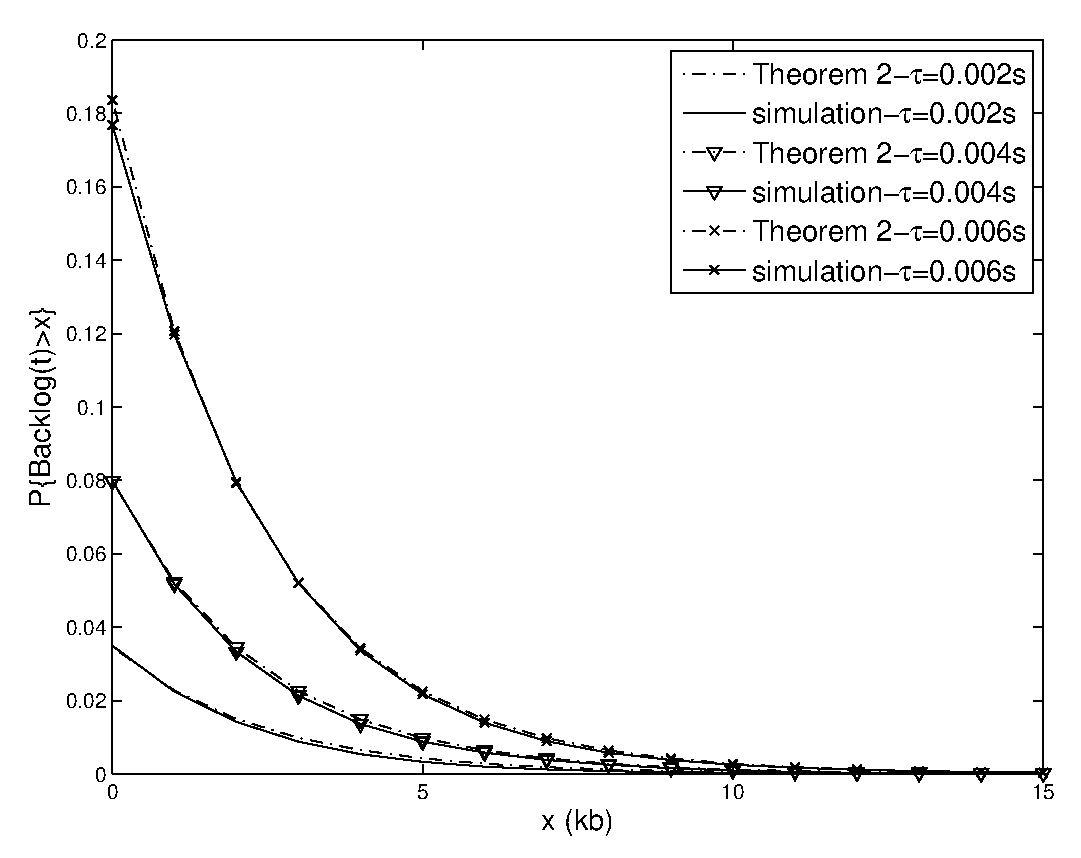
\includegraphics[scale=0.45]{figures/backlogtau.eps}\\
  \caption{Backlog Bound at $t=0$ for Scenario I}\label{backlogtau}
\end{figure}

\subsection{Scenario II}\label{scenario2}
In this subsection, we consider a special case of our flow control model, i.e. $C_2=+\infty$ and $\tau=0$. Under this condition, the equivalent service process $\mathcal{S}(t)$ is equal to the feed-forward service process $\mathcal{S}_1$. This scenario has been discussed in subsection 3.3 of \cite{jung1996analysis}, and the stationary probability $P\{\mathcal{L}=i\}$ was derived. The backlog bound can be calculated based on this probability, which is
\begin{eqnarray}\label{oldresult}
P\{\mathcal{L}>x\}&=&\sum_{i=x+1}^\infty P\{\mathcal{L}=i\}\nonumber\\
&=& P(0,0)\times\rho^{(W+x+1)}/(1-\rho)
\end{eqnarray}
where $\rho=\lambda/\mu$ and $P(0,0)=1/(1+\sum_{i=1}^W\rho^i+\rho^{W+1}/(1-\rho))$.

Due to the independent and stationary properties of arrival and service process, we can apply Theorem \ref{theorem3} to obtain the follow backlog bound
\begin{equation}\label{newresult}
P\{\mathcal{L}>x\}\leq e^{-\theta(W+x)}e^{\lambda(e^{\theta L}-1)+\mu(e^{-\theta L}-1)}
\end{equation}
where the free parameter $\theta$ satisfying $E[e^{\theta(\mathcal{A}(1)-\mathcal{S}(1))}]\leq 1$.

Let $\lambda=800s^{-1}$, $\mu=1000s^{-1}$, $\tau=0$ and $L=1kb$. We change the window size $W$ from $5kb$ to $15kb$, and present the numerical results calculated with Eq.(\ref{oldresult}) and Eq.(\ref{newresult}) in Fig. \ref{result3}. As shown in Fig. \ref{result3}, the backlog bound given in this paper is as tight as that given in \cite{jung1996analysis}, which is also the exact distribution of the backlog bound. This comparison indicates that our theorems can provide the same backlog bound as queueing theory. It is also worth highlighting that our theorems can be applied to much more general case, without restricting the arrival and service processes to be Markovian as the queueing theory based method does.
\begin{figure}
  \centering
  % Requires \usepackage{graphicx}
  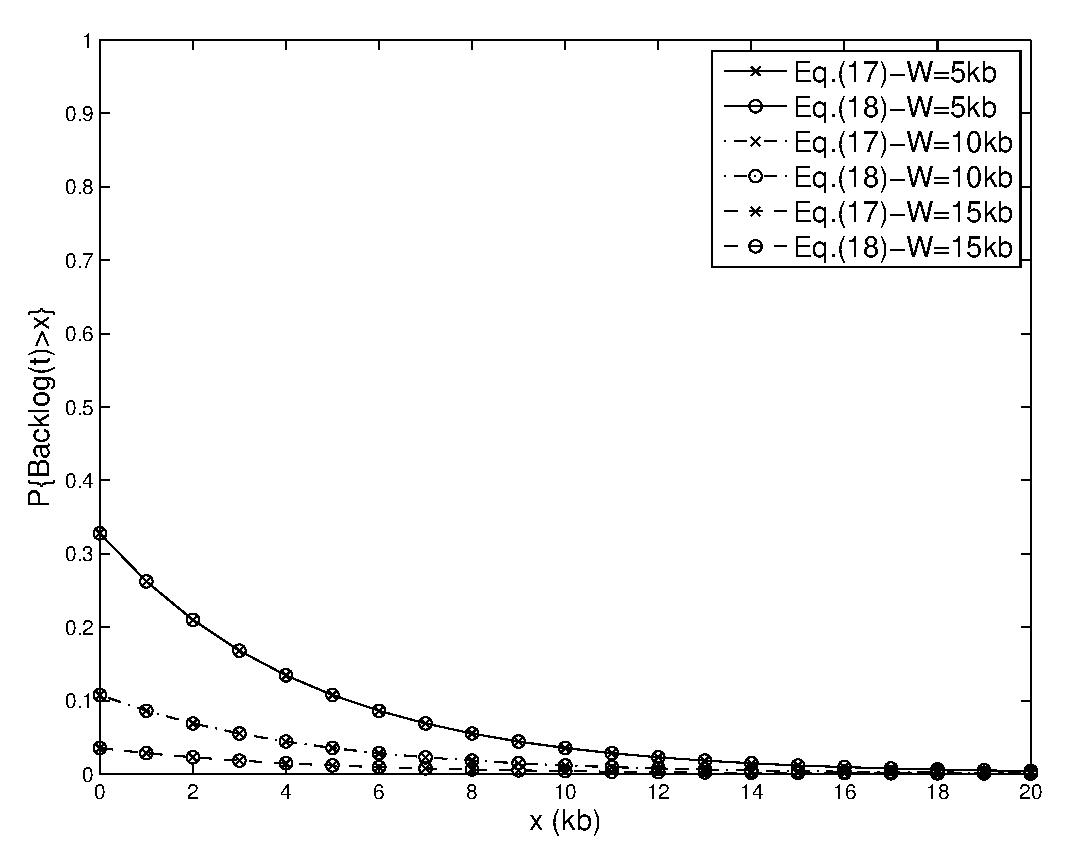
\includegraphics[scale=0.45]{figures/backlogcomp.eps}\\
  \caption{Backlog Bound for Scenario II}\label{result3}
\end{figure}

\subsection{Scenario III}
For this scenario, suppose the time is divided into slots with the same length $T$, and all the packets have the same length $L$. For each time slot, the source generates a packet with probability $p$ and keeps silent with probability $1-p$. Thus, arrival process $\mathcal{A}(t)$ is a typical two-states Markov-Modulated process. We can obtain the backlog bound with Theorem \ref{theorem2} or Theorem \ref{theorem3}, because the arrival and service processes of this scenario are both independent and stationary increment process. To demonstrate the tightness of Theorem \ref{theorem2} and Theorem \ref{theorem3}, we consider the follow two cases:

(1) $C_2=+\infty$ and $\tau=0$: For this case, the service process $\mathcal{S}(t)$ is equal to the feed-forward service process $\mathcal{S}_1(t)$, which is a Markovian process with exponentially distributed service time. We can obtain n backlog bound by applying Theorem \ref{theorem3}, which is
\begin{equation*}\label{equation3}
P\{\mathcal{L}(t)>x\}\leq e^{-\theta(W+x)}\cdot e^{\mu(e^{-\theta L}-1)+(1-p+pe^{\theta L})}
\end{equation*}
where $\theta>0$ and satisfying $\mu(e^{-\theta L}-1)+(1-p+pe^{\theta L})\leq 0$.

To verify the tightness of our theorem, we built an event-driven simulator based on the OMNeT++ discrete event simulation platform \cite{omnetpp}. Let $L=1kb$, $\mu=40s^{-1}$, $T=0.02s$, and change the window size from $5kb$ to $20kb$, we get the analytical results and simulation results. As shown in Fig. \ref{result1}, the analytical results match well with the simulation results, which indicates that, our theoretical bounds based on SNC can indeed predicate the performance of WFC exactly. Another observation is that, the backlog bound decreases along with the increasing of window size. However, the larger window size, the larger risk of network congestion. Hence, there is a tradeoff between the cost of buffer space and the risk of network congestion.
\begin{figure}
  \centering
  % Requires \usepackage{graphicx}
  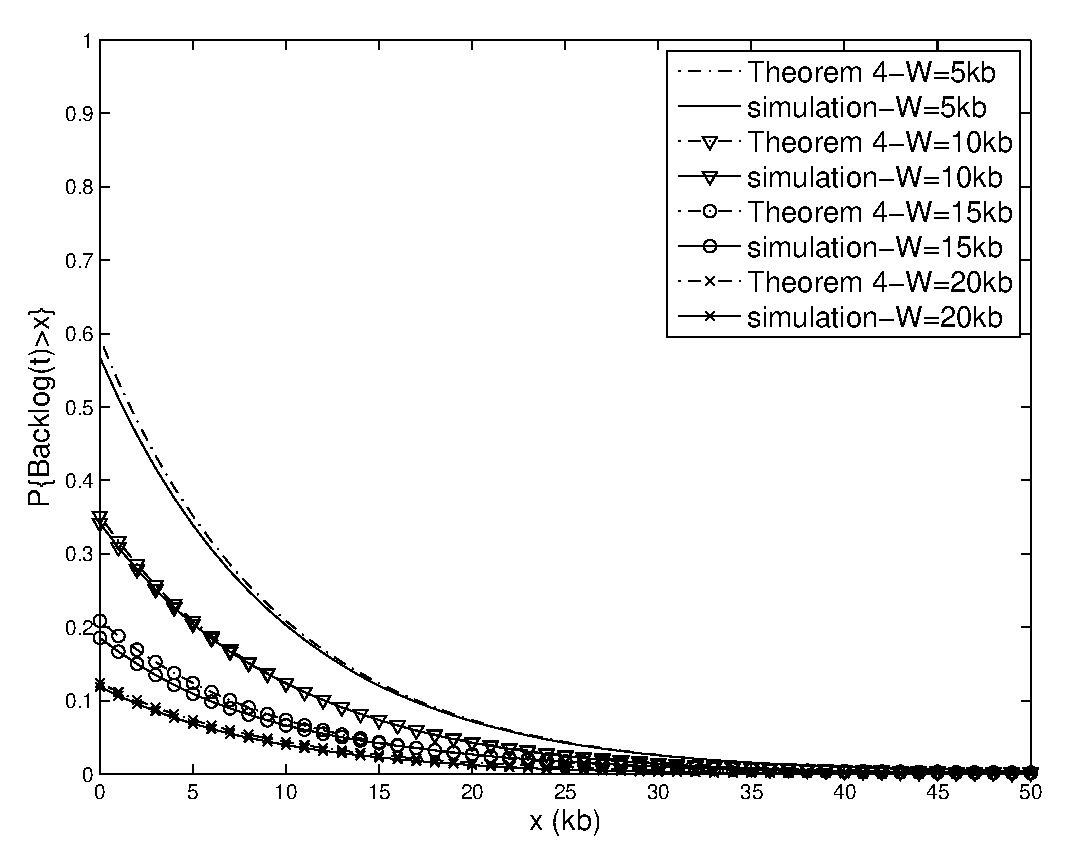
\includegraphics[scale=0.45]{figures/backlogbuf.eps}\\
  \caption{Backlog Bound for Scenario III with different Window Size}\label{result1}
\end{figure}

(2) $C_2<+\infty$ and $\tau> 0$: For this scenario, the arrival and service processes are stationary. The effective bandwidth of the arrival process can be found in \cite{Chan94}, i.e. $\rho(\theta,t)=\frac{1}{\theta}\log(1-p+pe^{\theta L})$. The effective capacity of the feed-back service process is $\mu_2^\prime(\theta)=C_2$, feed-forward service process $\mathcal{S}_1(t)$ provides exponentially distributed service time with parameter $\mu$ for each packet. Thus, the effective capacity of this service process with parameter $\mu$ is
\begin{eqnarray*}
\mu_1^\prime(\theta,t)&=& \frac{1}{-\theta t}log E[e^{-\theta \mathcal{S}_1(t)}]\\
&=& \frac{1}{-\theta t}log(\sum_{x=0}^\infty e^{-\theta Lx}\frac{e^{-t\mu}(t\mu)^x}{x!})\\
&=& \frac{\mu}{-\theta}(e^{-\theta L}-1).
\end{eqnarray*}

We can get a backlog bound by applying Theorem \ref{theorem2}, which is
\begin{equation}\label{bernoullibound}
P\{\mathcal{L}(t)>x\}\leq {t+2\choose 3}\cdot e^{-\theta [x+W-t/\theta log(1-p+pe^{\theta L})]}.
\end{equation}
This backlog bound can be minimized by selecting free parameters $\theta$ satisfying the following stability condition
\begin{equation}\label{stabilitycond3}
\rho(\theta)\leq \mu_1^\prime\otimes\mu_2^\prime(\theta).
\end{equation}

It is intuitive that a heavy offered load will lead to a large backlog bound, and our results  provide a way to quantitatively analyze the relationship between offered load and the backlog bound. To explore the impact of offered load on the backlog bound, we set $L=1kb$, $T=0.02s$, $W=5kb$, $\mu=50s^{-1}$, $\tau=0.002s$ and change the offered load by increasing the probability $p$ from $0.8$ to $0.95$. Figure \ref{result2} illustrates the calculated backlog bound of WFC at time instance $t=0.002s$. The numerical results was conducted by selecting appropriate $\theta$ under the constraint of Eq.(\ref{stabilitycond3}) to make the Eq.(\ref{bernoullibound}) as small as possible.
\begin{figure}
  \centering
  % Requires \usepackage{graphicx}
  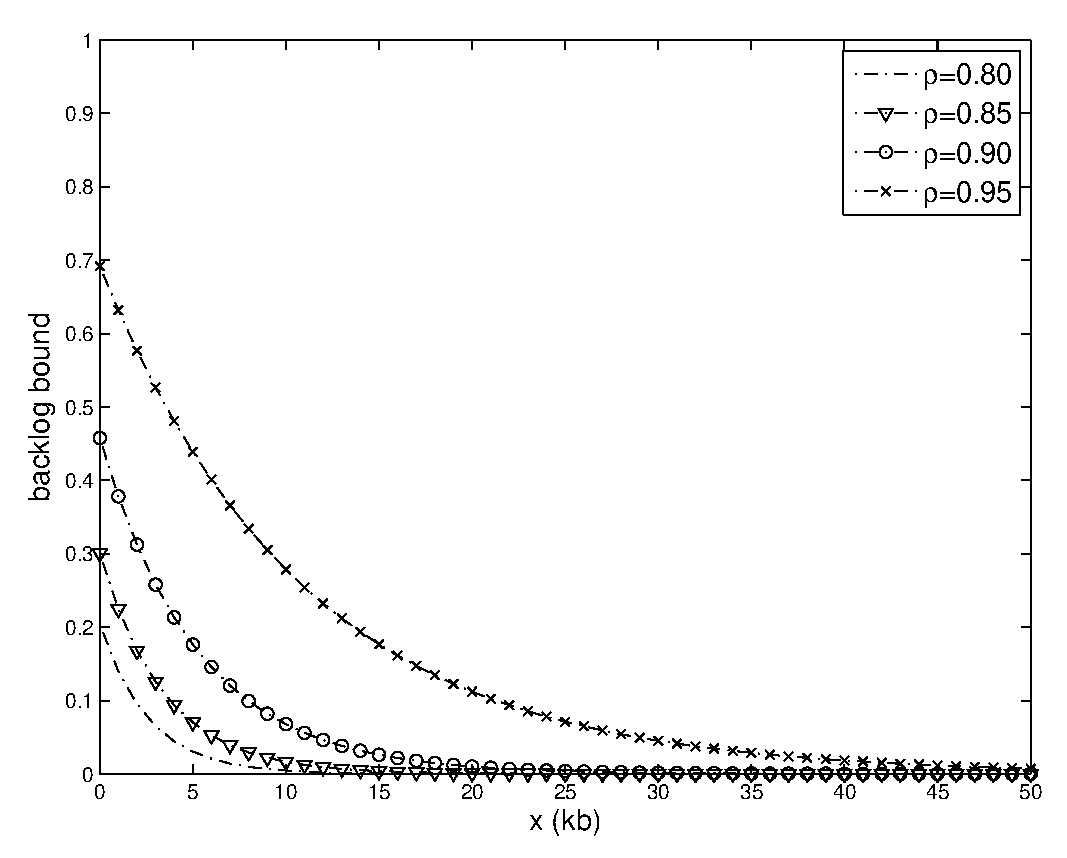
\includegraphics[scale=0.45]{figures/backlogrho.eps}\\
  \caption{Backlog Bound for Scenario III with different Offered Load}\label{result2}
\end{figure}

\section{Conclusion}\label{concluson}
Flow control has been widely used in the computer network to avoid network congestion, deadlock and unfair resource allocation. In this paper, we proposed a Stochastic Network Calculus (SNC) based performance model to evaluate the backlog bound of lossless Window Flow Controller (WFC). The derivation is conducted by leveraging the concept of beginning of last backlogged period and some advanced probability techniques, e.g. effective bandwidth, effective capacity and martingale. Given the WFC parameters (i.e. feedback delay and window size) and the traffic and service characterizations, our analytical framework can answer question related to the backlog bound of the controller. Our work is not only the stochastic extension for the previous research on the performance analysis of WFC with Deterministic Network Calculus (DNC), but also the generalization of the existing queueing theory based performance model. In addition, the influence of different WFC parameters on the backlog bound are also investigated. In the future work, we expect to extend these results to support the hop-by-hop window flow control.

\section*{Acknowledgment}
The authors would thank the reviewers for their suggestions and comments, and the first author would thanks Prof. Yuming Jiang of Norwegian University of Science and Technology (NTNU) for the fruitful discussion on the stochastic network calculus theory. This research is supported by High Technology Research and Development Program of China (Grant No. 2012AA012201, 2012AA011902).

\bibliographystyle{plain}% bib style
\bibliography{Docear}% your bib database

\end{document}
